
\documentclass[a4paper,11pt,oneside]{book}


\usepackage{fullpage}

\setlength{\topmargin}{-1cm}
\setlength{\headsep}{.5cm}
%\setlength{\footskip}{1.0cm}
\setlength{\textheight}{25.3cm}
\setlength{\textwidth}{17cm}
\setlength{\evensidemargin}{-.5cm}
\setlength{\oddsidemargin}{-.5cm}

\usepackage{pdfpages}
\usepackage[english]{babel}
\usepackage{amssymb,amsmath}
\usepackage[T1]{fontenc}
\usepackage{times} 
  
\usepackage{url}
  
\usepackage{fancyhdr}
\renewcommand{\footrulewidth}{0.4pt}
\pagestyle{fancy}
\lhead{Proceedings of the 17th Irish Machine Vision and Image Processing conference }
\rhead{IMVIP 2015}
\lfoot{August 26th-28th, 2016, Trinity College Dublin}
\cfoot{\thepage}
\rfoot{ISBN XXX-X-XXXXXXX-X-X}

\newif\ifpdf
  \ifx\pdfoutput\undefined
     \pdffalse
\else
  \pdfoutput=1
  \pdftrue
\fi \ifpdf
  \pdfcompresslevel=9
  \usepackage[pdftex]{hyperref}
  \hypersetup{backref,bookmarks=true,pdfpagemode=Fullscreen,linkcolor=black,colorlinks=true,urlcolor=blue}

        
\else
  \usepackage{graphicx}
\fi


\addtocounter{secnumdepth}{1}

\begin{document}

\thispagestyle{empty}

\includepdf[scale=1,pages=-]{frontpage.pdf}

\frontmatter

\chapter{Welcome }


This template creates table of content for the PDF documents (e.g. like conference proceedings) that are inserted as chapters in this book. The PDF template for the IMVIP proceedings is here inserted twice. 

The latex files are available at:
\begin{itemize}
\item  book template: \url{https://www.overleaf.com/read/wygmfbmrhyvt}

\item proceeding  template: \url{https://www.overleaf.com/read/snqwxxdpxbcn}
  
\end{itemize}
These templates were  created by the Irish Pattern Recognition and Classification Society \url{http://iprcs.org} and used first for  the 2015 IMVIP conference book of proceedings (available at \url{http://hdl.handle.net/2262/74714} as example).


%%%%%%%%%

\renewcommand{\contentsname}{Table of Contents}
\tableofcontents \pagestyle{fancy}

\mainmatter 

\includepdf[pages=-,addtotoc={1,chapter,0, Author Instructions for IMVIP 2015 \\ \textit{\textmd{R. Dahyot \& K. Dawson-Howe}},1},pagecommand={\pagestyle{fancy}}]{imvip2015_Formatting_Instructions.pdf}


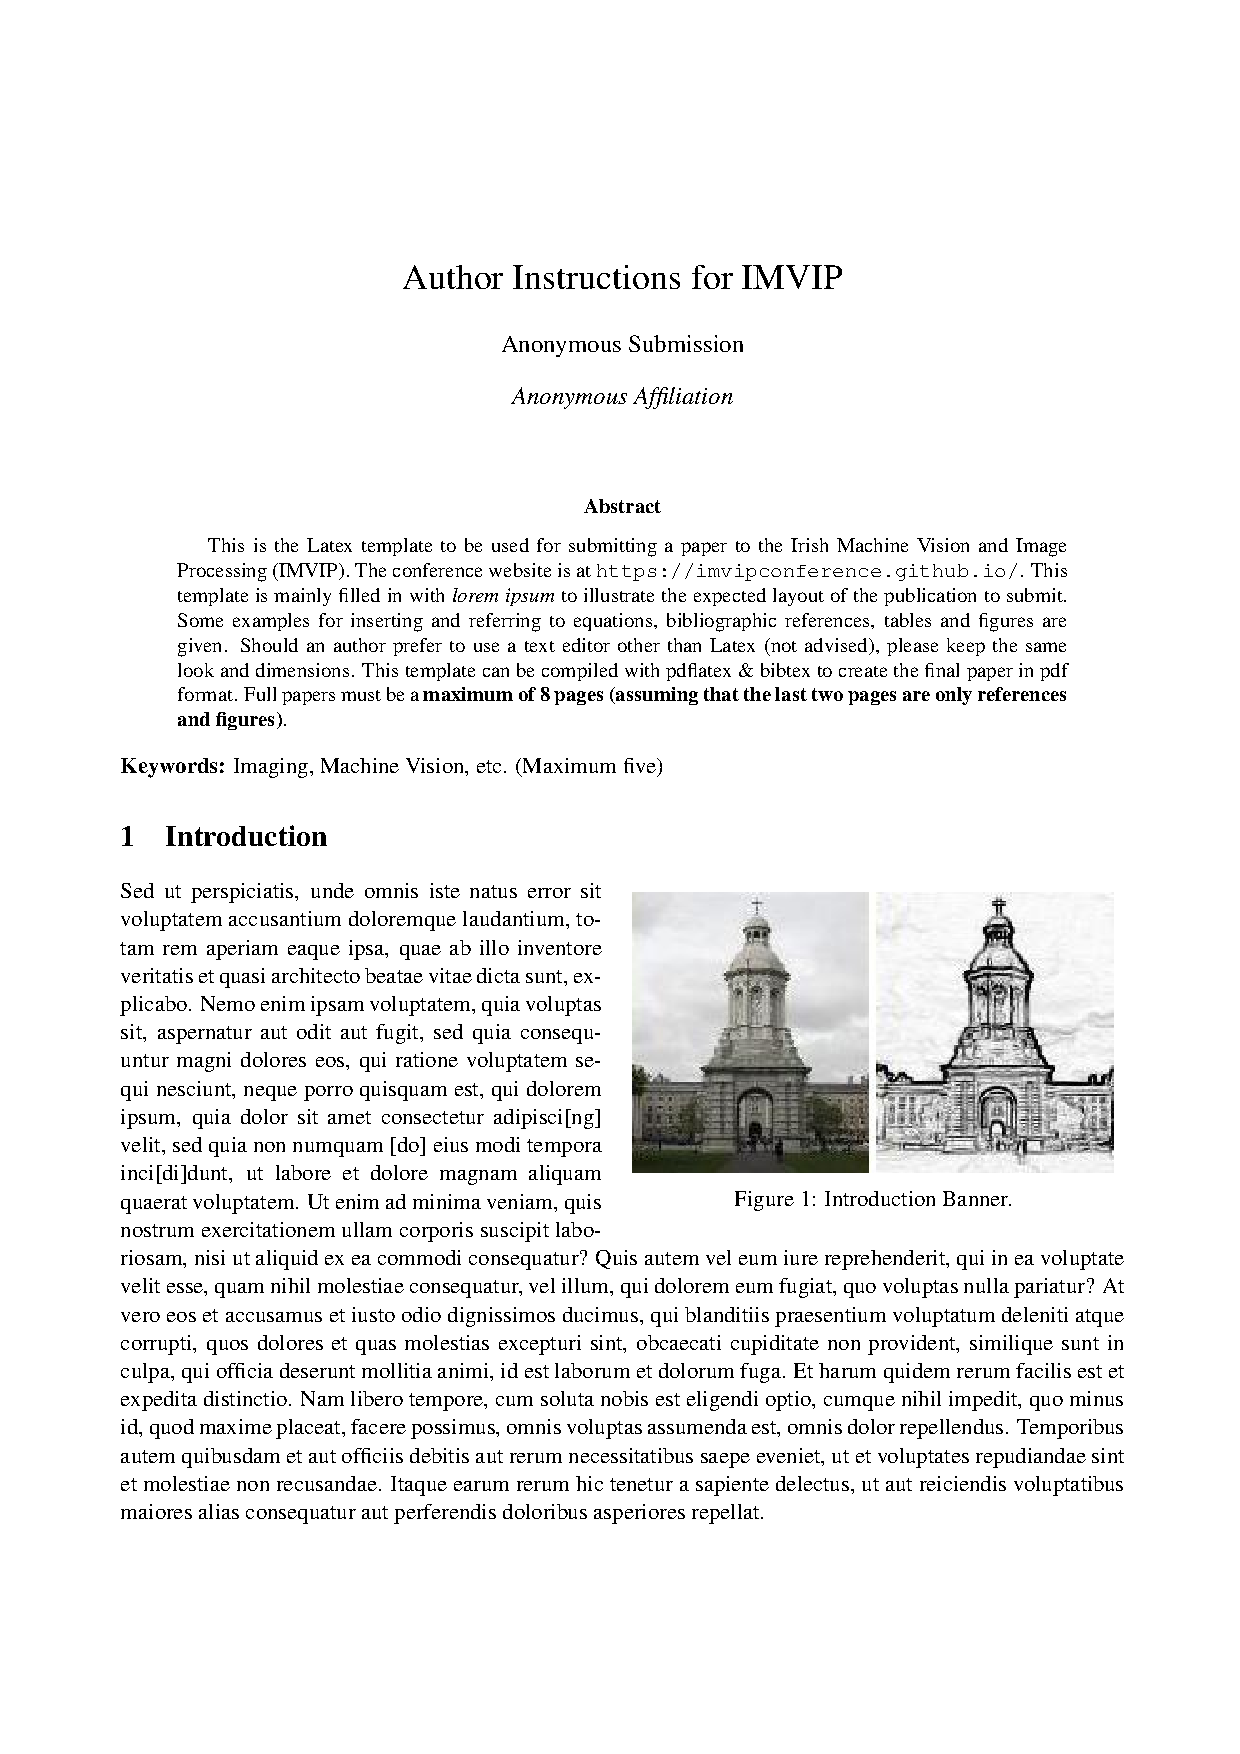
\includepdf[pages=-,addtotoc={1,chapter,0, Author Instructions for IMVIP 2015 \\ \textit{\textmd{R. Dahyot \& K. Dawson-Howe}},1},pagecommand={\pagestyle{fancy}}]{imvip_Formatting_Instructions.pdf}



%%%%%%%%%
\backmatter
\thispagestyle{empty}

\includepdf[scale=1,pages=1]{backpage.pdf}


\end{document}
